
% This work is licensed under the Creative Commons Attribution-Share Alike 2.0 France License.
% To view a copy of this license, visit http://creativecommons.org/licenses/by-sa/2.0/fr/legalcode
% or send a letter to Creative Commons, 171 Second Street, Suite 300, San Francisco, California, 94105, USA.


\scalefont{0.8}
\ChNumVar{\fontsize{100}{100}\selectfont\textit} 
%\ChNameVar{\fontsize{5}{5}\selectfont\textrm} 
\ChTitleVar{\fontsize{28}{28}\selectfont\textrm}

\frontmatter

%\lstset{language=Python}
%\addfontfeature{Ligatures=Historical}

%\addfontfeature{Numbers=OldStyle}

\addfontfeature{Fractions=On}
\thispagestyle{empty}



\begin{center}
\textcolor{bleu}{\textbf{\fontsize{40}{40}\selectfont\textsf{Domptage de serpent pour les enfants}}}

\textcolor{bleu}{\textsf{\begin{Huge}Apprendre à programmer avec Python\end{Huge}}}

\vspace{1cm}

\begin{flushleft}
\textcolor{red}{\textsf{\begin{Huge}\Ovalbox{Édition 
 \begin{WINDOWS}Windows\end{WINDOWS}
 \begin{LINUX}Linux\end{LINUX}
 \begin{MAC}Mac Os X\end{MAC} 
}\end{Huge}}}
\end{flushleft}

\AddToShipoutPicture*{
 \put(0,0){
 \parbox[b][\paperheight]{\paperwidth}{
 \vfill
 \vspace{2cm}
\begin{flushleft}
\hspace*{0cm}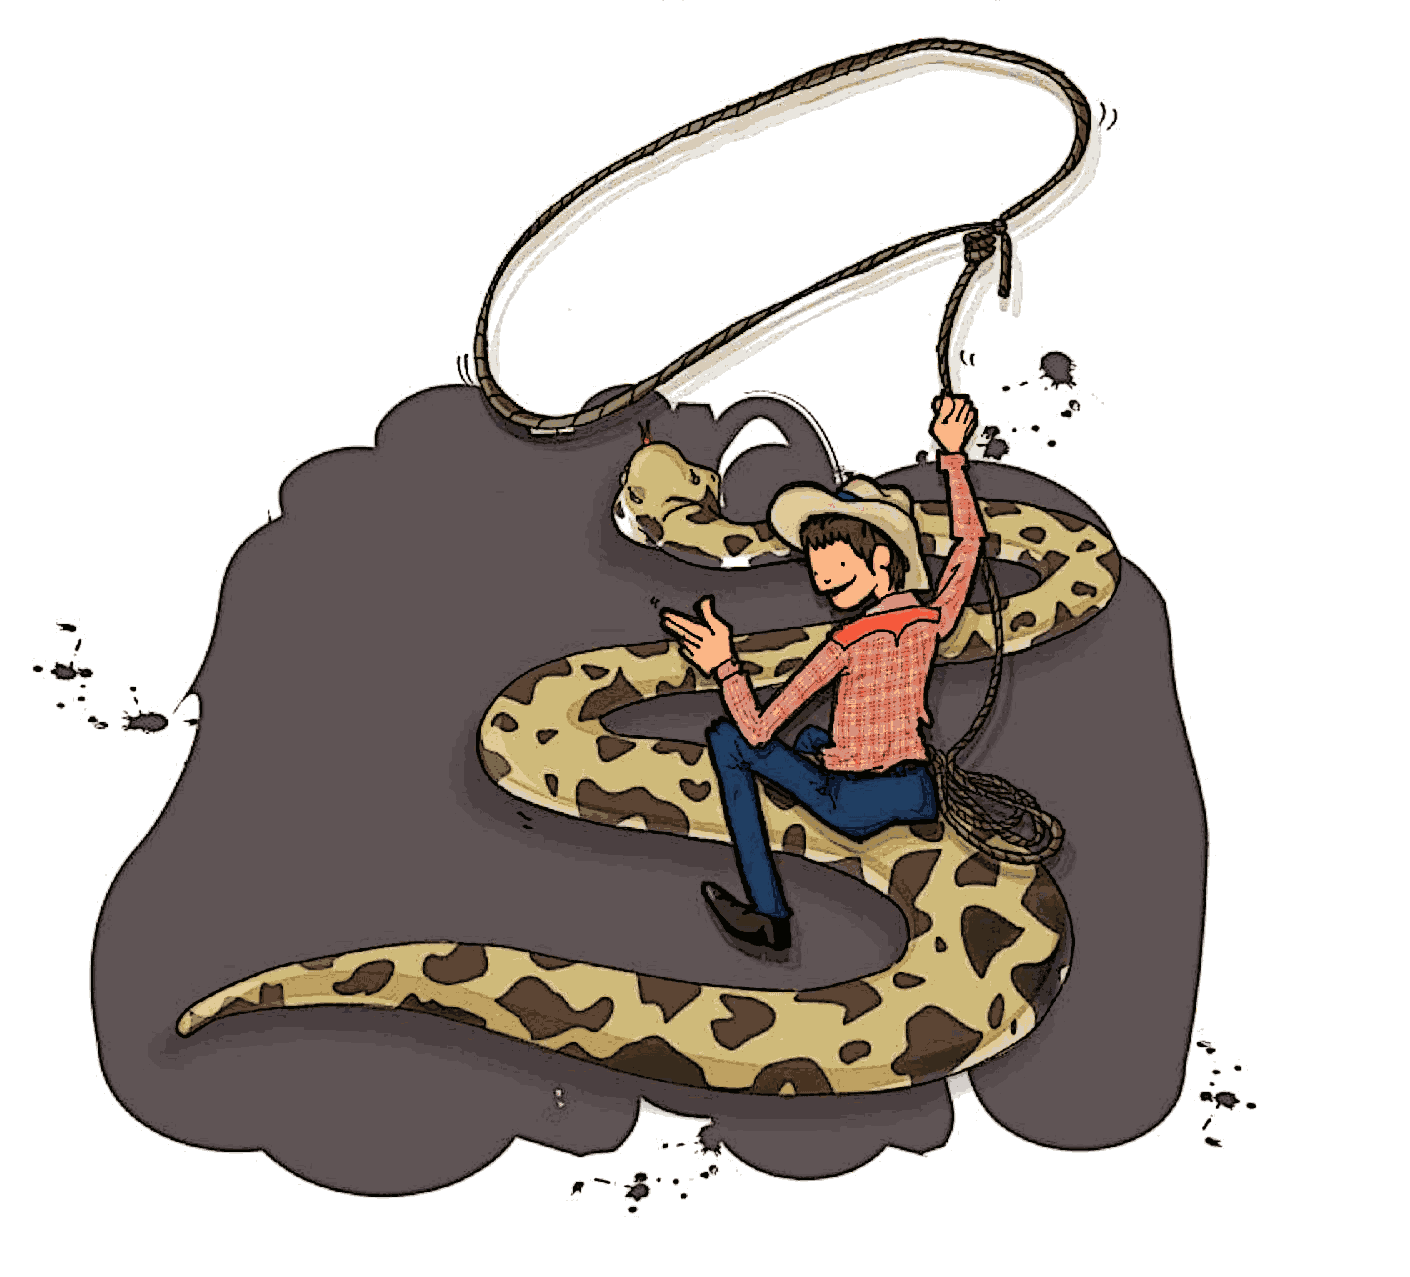
\includegraphics[width=20cm]{images/couv.png}
\end{flushleft}
 \vfill
 }}}

\vspace{16cm}

%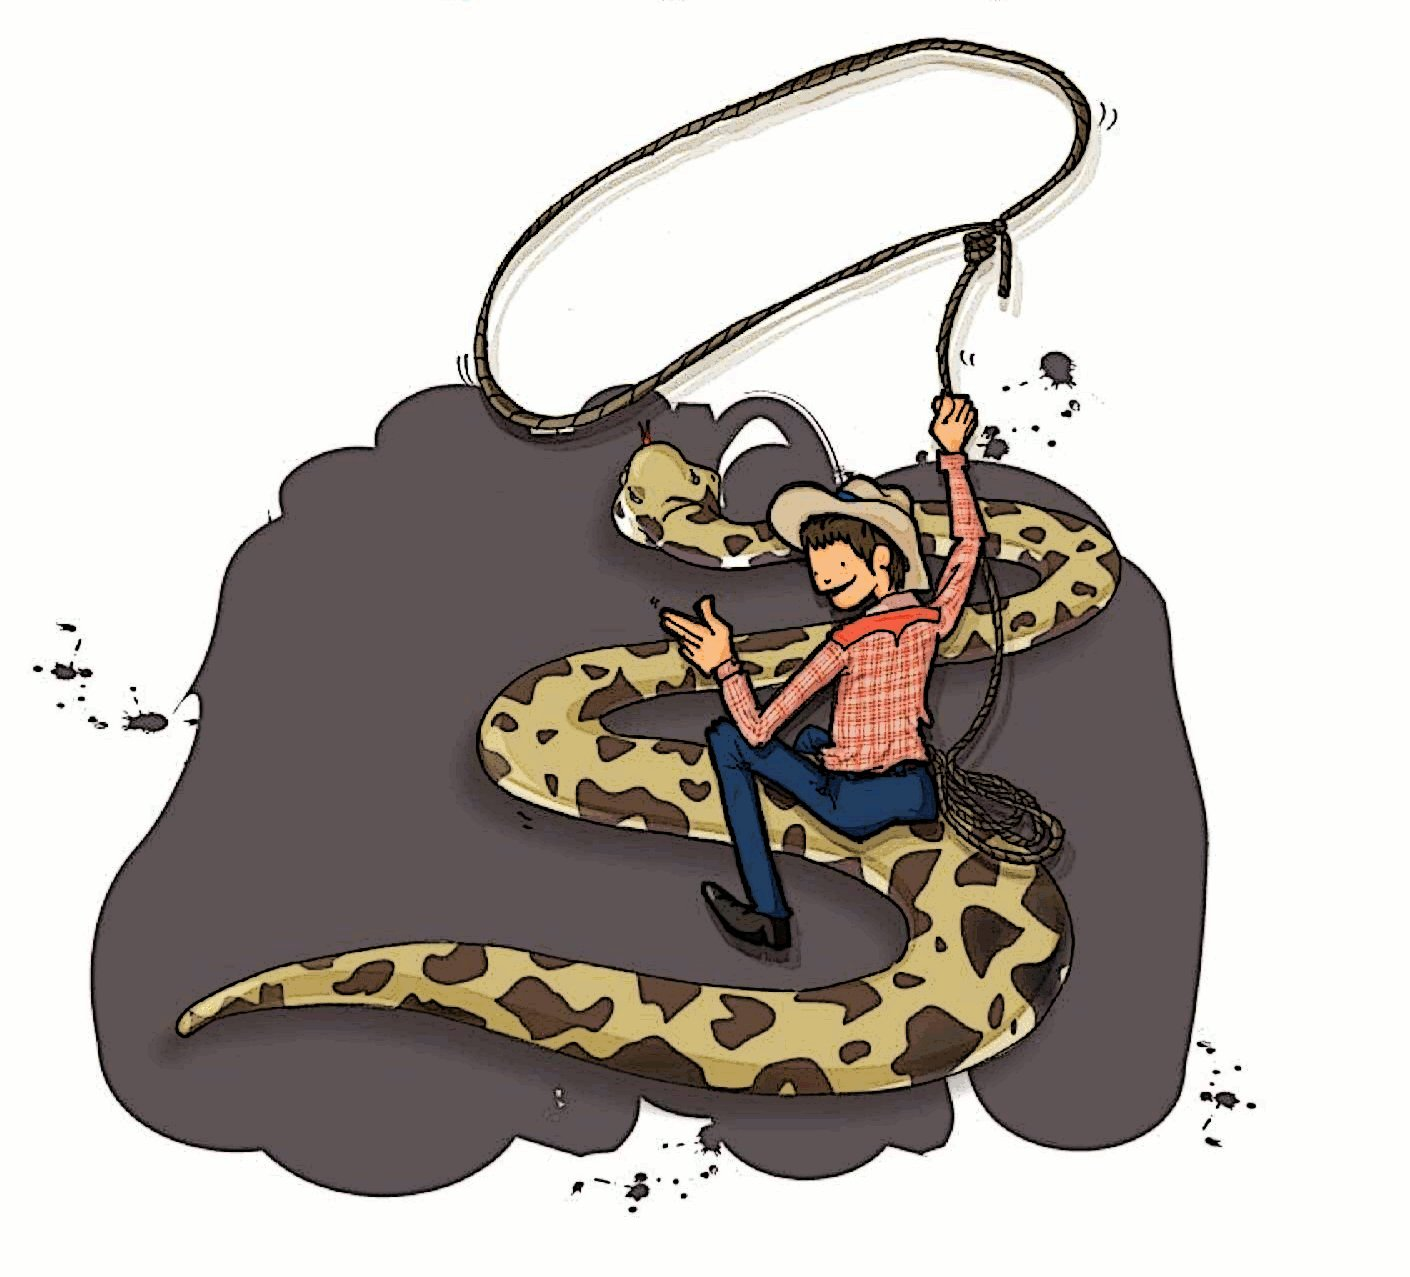
\includegraphics[scale=0.35]{images/couv.jpg} 
\end{center}

\begin{flushright}
\textcolor{bleu}{\begin{Huge}\textsf{Écrit par Jason R. Briggs}\end{Huge}}

\textcolor{bleu}{\begin{huge}\textsf{Traduit et adapté par Michel Weinachter}\end{huge}}
\end{flushright}

\newpage

\textit{Domptage de serpent pour les enfants, apprendre à programmer en Python}

par Jason R. Briggs

traduit et adapté par Michel Weinachter

\bigskip
Version: 0.7.7

Version française: 0.0.9

\bigskip
Copyright © 2007-2009

\bigskip
Publié par... ah, personne en fait.

\bigskip
Remarques: \href{mailto:livres@weinachter.com?subject=Domptage de serpents pour les enfants}{livres@weinachter.com}

\bigskip
L'ensemble des illustrations créées ou modifiées pour la traduction ont été faites en utilisant \emph{the GIMP} et \emph{Inkscape}.
Illustration de couverture par Nuthapitol C., illustrations par Nuthapitol C. et Michel Weinachter, cliparts:
\url{http://openclipart.org} et \url{http://commons.wikimedia.org}. 

\bigskip
Édité avec \TeX{}{\fontspec{Linux Libertine O C}\textbf{\emph{Maker}}} majoritairement sous Gnu/Linux et quelquefois en utilisant Portable Keyboard Layout (avec une disposition fr-oss) sous Windows.
 
Composé avec \XeTeX{} et \XeLaTeX{} en utilisant les fontes \emph{Linux Libertine}, \textsf{Linux Biolinum}, \texttt{Computer Modern}, \setsansfont[Mapping=tex-text]{DejaVu Sans}\textsf{DejaVu} pour quelques symboles, et Firefly pour quatre caractères chinois {\fontspec{AR PL UMing CN}漢字}.%\zhfont{漢字}.
 
\bigskip
Site web:

\url{http://www.briggs.net.nz/log/writing/snake-wrangling-for-kids}

\bigskip
Remerciements de l'auteur: merci à Guido van Rossum (pour la bienveillante dictature du langage Python), les membres de la liste de diffusion Edu-Sig (pour leurs avis et commentaires utiles) et à l'auteur David Brin (l'instigateur original de ce livre).

\bigskip
Remerciements du traducteur: merci à Jason R. Briggs, Gael Lickindorf, Anne, Christophe, Thaïs \& Anne-Sophie.

\bigskip
\begin{center}

%\begin{tabular}[t]{cc}
Licence:
%&


\includegraphics[scale=0.4]{images/CC-BY-SA.png}\\ 
%\end{tabular} 

\end{center}


Cette Œuvre est licenciée selon les termes du Contrat Public Creative Commons: 
Paternité-Partage des Conditions Initiales à l'Identique 2.0 France
Pour voir une copie de cette licence vous pouvez vous rendre à l'adresse suivante:
\url{http://creativecommons.org/licenses/by-sa/2.0/fr/}.

\bigskip

Vous êtes libres:
\begin{description}

\item[] 
\includegraphics[scale=0.2]{images/Share.pdf}\bf{} de reproduire\rm, distribuer et communiquer cette création au public
\item[] 
\includegraphics[scale=0.2]{images/remix.pdf}\bf{} de modifier\rm{} cette création
\end{description}

\bigskip
Selon les conditions suivantes:
\begin{description}
\item[] 
\includegraphics[scale=0.2]{images/Cc-by_new.pdf}\bf{} Paternité\rm{}. Vous devez citer le nom de l'auteur original de la manière indiquée par l'auteur de l'œuvre ou le titulaire des droits qui vous confère cette autorisation (mais pas d'une manière qui suggérerait qu'ils vous soutiennent ou approuvent votre utilisation de l'œuvre).
\item[] 
\includegraphics[scale=0.2]{images/sa.pdf} \textbf{Partage des Conditions Initiales à l'Identique}. Si vous modifiez, transformez ou adaptez cette création, vous n'avez le droit de distribuer la création qui en résulte que sous un contrat identique à celui-ci.
\end{description}
\begin{itemize}
\item À chaque réutilisation ou distribution de cette création, vous devez faire apparaître clairement au public
les conditions contractuelles de sa mise à disposition. La meilleure manière de les indiquer est un lien vers la
 page web:\\
\url{http://creativecommons.org/licenses/by-sa/2.0/fr/}.

\item Chacune de ces conditions peut être levée si vous obtenez l'autorisation du titulaire des droits sur cette œuvre.
\item Rien dans ce contrat ne diminue ou ne restreint le droit moral de l'auteur ou des auteurs.
\end{itemize}

\bigskip
Ce qui précède n'affecte en rien vos droits en tant qu'utilisateur (exceptions au droit d'auteur: copies réservées à l'usage privé du copiste, courtes citations, parodie...).

Une version complète du Contrat est disponible sur:\\
\url{http://creativecommons.org/licenses/by-sa/2.0/fr/legalcode}.

\scalefont{1.4}
\sommaire

\vfill
\begin{center}
 
\includegraphics[width=5cm]{images/logo_afpy_v3.pdf}
\end{center}
\vfill



%\clearpage
%\newpage
%\AddToShipoutPicture*{\BackgroundPicture}
%\phantom{a}
%\vspace{9cm}
% \begin{center}
%\fontsize{50}{50}\selectfont
%\textcolor{gray}{\XeTeX}
%\end{center}
%\vfill
